\documentclass[11pt]{article}

% parameters are fairly self-explanatory here, thankfully
\usepackage[width=7in,height=9.5in,top=0.75in,centering]{geometry}

% for math-ing
\usepackage{amsmath}
\usepackage{amssymb}


%%%%%% tables %%%%%%%%

\usepackage{array}
\renewcommand{\arraystretch}{1.5}
\setlength{\tabcolsep}{8pt}

%%%%%% plotting %%%%%%

\usepackage[dvipsnames]{xcolor}
\usepackage{tikz}
\usepackage{pgfplots}

\pgfplotsset{every axis/.append style={
                    axis x line=middle,    % put the x axis in the middle
                    axis y line=middle,    % put the y axis in the middle
                    axis line style={<->,color=black}, % arrows on the axis
                    xlabel={$x$},          % default put x on x-axis
                    ylabel={$y$},          % default put y on y-axis
            }}
            
 \pgfplotsset{compat=1.14} % sometimes, everything falls apart without this
 
 %\usepgfplotslibrary{fillbetween} %for shading between curves

%%%%%% commands %%%%%%

% exam heading; course name is first argument, exam information is second argument
\newcommand{\Heading}[2]{
    \fbox{
        {\Large\textbf{#1}}
        }
    \hfill
    \fbox{
        \begin{minipage}{0.2\textwidth}
            \begin{center}
            \textbf{#2}
            \end{center}
        \end{minipage}
    }
    \par\vspace{0.1in}}

% for being lazy while beautifying integrals
\newcommand{\dint}{\displaystyle\int}

% for being lazy while beautifying limits
\newcommand{\dlim}{\displaystyle\lim}

%%%%%% stuff %%%%%%

\usepackage{fancyhdr}

%\setcounter{page}{0} % first page is page 0

\parindent0pt % no indent

\fboxsep=0.25cm % little space in fbox border

%%%%%% BEGIN! %%%%%%%

\begin{document}

\pagestyle{fancy}

% record goals here to create sense of transparency

\fancyhead[c]{%
  \ifcase\value{page}
  % empty test for page = 0
  \or {}% 
  \or
  \or {\bf\color{ProcessBlue} F2: Exponential and Logarithmic Functions}% page=1
  \or {\bf\color{ForestGreen} D3: Derivatives of Basic Functions}% page = 2
  \or {\bf\color{ForestGreen} D2: Compute Derivatives}% page = 3
  \or {\bf\color{RedOrange} A1: Derivatives and Graphing}% page = 4
  \or {\bf\color{RedOrange} A2: Local and Absolute Extreme Values}% page = 5
  \or {\bf\color{RedOrange} A3: Applied Optimization}% page = 6
  \or {\bf\color{RedOrange} A3: Applied Optimization}% page = 6
  \or {\bf\color{Fuchsia} I1: Meaning of an Integral}% page = 7
  \or {\bf\color{Fuchsia} I2: Properties of Definite Integrals}% page = 8
  \or
  \else
  % Empty chead here!
  \fi
}

\thispagestyle{empty} % don't display that this is page 0

\Heading{MATH 1190/1210 Survey of Calculus I}{Knowledge Checkpoint 3\\ Solutions\\Fall 2025}

\vspace{0.1in}

\textbf{Name} \hrulefill \, \begin{minipage}{0.16\textwidth}\begin{center}\textbf{UVA ID\\ (e.g. hdj4nd)} \end{center}\end{minipage}\hrulefill\\

\begin{minipage}{0.2\textwidth}\begin{center}\textbf{Course \&\\ Section Number} \end{center}\end{minipage} \hrulefill\,\,\textbf{Date} \hrulefill  \\

\hrulefill
\paragraph*{Course \& Section Numbers:}

{\small
\begin{center}
\begin{tabular}{| c | c | c | c | c |}
\hline
%
\begin{minipage}{0.12\textwidth}\begin{center}
1190-100\\
J. Rolf\\
(11:00 AM)
\end{center}\end{minipage}
&
\begin{minipage}{0.12\textwidth}\begin{center}
1190-200\\
J. Rolf\\
(9:30 AM)
\end{center}\end{minipage}
&
\begin{minipage}{0.12\textwidth}\begin{center}
1210-100\\
Mikhail\\
(8 AM)
\end{center}\end{minipage}
&
\begin{minipage}{0.12\textwidth}\begin{center}
1210-200\\
Raul\\
(9:30 AM)
\end{center}\end{minipage}
&
\begin{minipage}{0.12\textwidth}\begin{center}
1210-300\\
Sherman\\
(11 AM)
\end{center}\end{minipage}
\\
%
\hline
%
\begin{minipage}{0.12\textwidth}\begin{center}
1210-400\\
Sherman\\
(12:30 PM)
\end{center}\end{minipage}
&
\begin{minipage}{0.12\textwidth}\begin{center}
1210-500\\
Michael\\
(2 PM)
\end{center}\end{minipage}
&
\begin{minipage}{0.12\textwidth}\begin{center}
1210-600\\
J. Bowling\\
(3:30 PM)
\end{center}\end{minipage}
&
\begin{minipage}{0.12\textwidth}\begin{center}
1210-700\\
Josh\\
(9:30 AM)
\end{center}\end{minipage}
&
\begin{minipage}{0.12\textwidth}\begin{center}
1210-800\\
Mason\\
(2 PM)
\end{center}\end{minipage}
\\
%
\hline
%
\begin{minipage}{0.12\textwidth}\begin{center}
1210-900\\
Caelan\\
(3:30 PM)
\end{center}\end{minipage}
&
\begin{minipage}{0.12\textwidth}\begin{center}
1210-920\\
Caelan\\
(5 PM)
\end{center}\end{minipage}
&
\begin{minipage}{0.12\textwidth}\begin{center}
1210-940\\
Mitchell\\
(10 AM)
\end{center}\end{minipage}
&
\begin{minipage}{0.12\textwidth}\begin{center}
1210-950\\
Mitchell\\
(11 AM)
\end{center}\end{minipage}
&
\begin{minipage}{0.12\textwidth}\begin{center}
1210-960\\
Mitchell\\
(noon)
\end{center}\end{minipage}
\\
\hline
\end{tabular}
\end{center}

}

{%\small

\paragraph*{Instructions:}

\begin{itemize}
    
    \item The regular time allowed for completing this assessment is \fbox{$80$} minutes.
    %\item This assessment is out of 50 points.\\
    \item This assessment contains one single-part or multi-part problem for each of the following targets:  {\bf\color{ProcessBlue}F2}, {\bf\color{ForestGreen}D3}, {\bf\color{ForestGreen}D2}, {\bf\color{RedOrange}A1}, {\bf\color{RedOrange}A2}, {\bf\color{RedOrange}A3}, {\bf\color{Fuchsia}I1}, {\bf\color{Fuchsia}I2}.
    \item On each problem, you will receive a score of Exceeds Expectations (5), Proficient (4), Almost (3), Developing (2), Emerging (1), or Not Yet (0). {\bf Please do not interpret your score as a percentage.}
    %\item You will have opportunities to reassess on the targets appearing on this assessment after the next {\bf 2} assessments.\\
    \item You may NOT use calculators, dictionaries, notes, phones, or any other kind of aid.
    \item Please write neatly. What cannot be read, cannot be graded.
    \item Carefully work out each problem and clearly indicate your final answer to every problem.
    \item Throughout, give the most descriptive answer possible. \textbf{For instance, ``DNE" will not be accepted when ``$=\infty$" is applicable.}
    %\item Please provide the most specific answer possible. For instance, if a limit does not exist because it goes to $\infty$ or $-\infty$, then specify this.
    \item Please use the methods discussed up to this point in the course. For example, any work based on l'H\^opital's Rule will not receive credit.
    \item \textbf{All work must be shown unless otherwise specified.} Partial credit will not be given if appropriate work is not shown.
    \item In particular, {\bf any answer appearing with no justification will receive no credit regardless of whether the answer was correct}, unless otherwise specified.
    \item Please first respond to the prompts on which you feel most proficient, then respond to others later.
    \item This booklet is printed double-sided. It contains 12 pages and 8 numbered problems.
    \item There's a formula sheet on the second-to-last page of common area/volume formulas and optimization concepts in case you need them.
    \end{itemize}
    
    }

\vfill


%%%%%%%%%
\newpage

This page is left blank intentionally.\\

Use this page if you need additional space to write your solutions to any problem. \\

If you wish this page graded, you must refer to this page on \textbf{the original page} of the problem. Otherwise, your grader will NOT consider your work on this page.

\newpage%
%%%%%%%%%


\begin{enumerate}

%%%%%%%%%%%%%%%%%%%%%%%%%%%%%%%%%%%%%%%%%%%%%%%%%%%%%
%%%%%%%%%%% BEGIN PROBLEM F2 %%%%%%%%%%%%%%%%%%%%%%%%
%%%%%%%%%%%%%%%%%%%%%%%%%%%%%%%%%%%%%%%%%%%%%%%%%%%%%

%properties of exponents
%logarithmic equations

\item Respond to the following prompts. 

\begin{enumerate}
    \item Fully simplify of the expressions below. Each of your final answers should be a number or expression without any exponents.

    \begin{enumerate}
        \item[(i)] $(\sqrt{5x^0})^{4}$, where $x$ is a positive real number. 
        \vspace{0.5cm}
        
{\color{blue}Solution: 
$(\sqrt{5x^0})^{4} = (\sqrt{5\cdot 1})^{4} = (\sqrt{5})^{4} = (5^{\frac{1}{2}})^{4} = (5^{\frac{4}{2}}) = (5^2) = 25$
}
        \vfill

        \item[(ii)] $\dfrac{2^{-4}\cdot3^2}{2^{-2}\cdot3^3}$

             \vspace{0.5cm}
        
{\color{blue}Solution: 
$\dfrac{2^{-4}\cdot3^2}{2^{-2}\cdot3^3} = 2^{-4 + 2}\cdot3^{2 - 3} = 2^{-2} \cdot 3^{-1} = \dfrac{1}{2^2 \cdot 3} = \dfrac{1}{4 \cdot 3} = \dfrac{1}{12}$
}
    \end{enumerate}

    \vfill

    \item Solve the following equation for $x$. 

    \[\log_3(2x^2+3)=2\]
             \vspace{0.5cm}
        
{\color{blue}Solution: 
\begin{align*}
\log_3(2x^2+3) &=2 \iff \\
3^{\log_3(2x^2+3)}&=3^{2} \iff\\
2x^2 + 3 &= 9 \iff\\
2x^2  &= 6 \iff\\
x^2 &= 3 \iff\\
x & = \pm \sqrt{3}
\end{align*}
Check: $x = \sqrt{3} \\
\log_3(2(\sqrt{3})^2+3) = \log_3(2\cdot 3+3) = \log_3(6+3) = \log_3(9) = 2  \ \checkmark$
\medskip

Check: $x = -\sqrt{3}\\
\log_3(2(-\sqrt{3})^2+3) = \log_3(2\cdot 3+3) = \log_3(6+3) = \log_3(9) = 2  \ \checkmark$
}
    \vfill
\end{enumerate}

%Show all work to support your final answer. In other words, if two expressions are equal, please show work to demonstrate why they are equal. If two expressions don't equal, please show why.

%\begin{itemize}
%    \item $\left(\dfrac{1}{5/3}\right)^{-2}$
%    \item $\left(\dfrac{5^{-2}}{3^{-2}}\right)$
    %\item $2\log\left(\dfrac{3}{5}\right)$
%\end{itemize}

%%%%%%%%%%%%%%%%%%%%%%%%%%%%%%%%%%%%%%%%%%%%%%%%%%%%%
%%%%%%%%%%% END PROBLEM F2 %%%%%%%%%%%%%%%%%%%%%%%%%%
%%%%%%%%%%%%%%%%%%%%%%%%%%%%%%%%%%%%%%%%%%%%%%%%%%%%%

\newpage

%%%%%%%%%%%%%%%%%%%%%%%%%%%%%%%%%%%%%%%%%%%%%%%%%%%%%
%%%%%%%%%%% BEGIN PROBLEM D3 %%%%%%%%%%%%%%%%%%%%%%%%
%%%%%%%%%%%%%%%%%%%%%%%%%%%%%%%%%%%%%%%%%%%%%%%%%%%%%

\item Write down the derivatives of the following functions. 

Although no work is required, you are highly encouraged to include any work that shows your thought process. 

\begin{center}
        \begin{tabular}{l c l l c l}
            %
            $\displaystyle\frac{d}{dx}\left[ \log_{1/3}(3) \right]$ & $=$ & {\color{blue} 0} &
            %
            %$\displaystyle\frac{d}{dx}\left[ 5x^3 \right]$ & $=$ & \rule[-8pt]{1.5in}{0.4pt}\\[0.3in]
            %%%%%
            %$\displaystyle\frac{d}{dx}\left[ \dfrac{4}{x^4} \right]$ & $=$ & \rule[-8pt]{1.5in}{0.4pt} & 
            %%%%%
            $\displaystyle\frac{d}{dx}\left[ 3e^x-\dfrac{4}{x^4} \right]$ & $=$ & {\color{blue} $3e^x+16x^{-5}$ }\\[1in]
            %%%%%
            $\displaystyle\frac{d}{dx}\left[ \log_9(x) \right]$ & $=$ & {\color{blue} $\displaystyle\frac{1}{x \cdot \ln 9}$} &
            %
            $\displaystyle\frac{d}{dx}\left[ \left(\dfrac{5}{2}\right)^x \right]$ & $=$ & {\color{blue} $\left(\displaystyle \frac{5}{2} \right)^x \cdot \ln\left( \displaystyle\frac{5}{2} \right)$}\\[1in]
            %%%%%
            $\displaystyle\frac{d}{dx}\left[ \dfrac{2x^8-10x}{x^2} \right]$ & $=$ & {\color{blue} $\displaystyle\frac{d}{dx}\left[2x^6 -10x^{-1}\right] = 12x^5+10x^{-2}$} & 
            %
            $\displaystyle\frac{d}{dx}\left[ 6\sqrt{x^3}-11 \right]$ & $=$ & {\color{blue}  $\displaystyle\frac{d}{dx}[ 6 x^{3/2} ] = 9\sqrt{x}$}\\[0.3in]
            %%%%%
        \end{tabular}
        
\end{center}

%%%%%%%%%%%%%%%%%%%%%%%%%%%%%%%%%%%%%%%%%%%%%%%%%%%%%
%%%%%%%%%%% END PROBLEM D3 %%%%%%%%%%%%%%%%%%%%%%%%%%
%%%%%%%%%%%%%%%%%%%%%%%%%%%%%%%%%%%%%%%%%%%%%%%%%%%%%

\newpage

%%%%%%%%%%%%%%%%%%%%%%%%%%%%%%%%%%%%%%%%%%%%%%%%%%%%%
%%%%%%%%%%% BEGIN PROBLEM D2 %%%%%%%%%%%%%%%%%%%%%%%%
%%%%%%%%%%%%%%%%%%%%%%%%%%%%%%%%%%%%%%%%%%%%%%%%%%%%%

\item Find the derivative of the following expressions. 

A correct final answer receives full credit. Nevertheless, you are encouraged to write down the steps so that you will be able to receive partial credit if you final answer is not fully correct. There's no need to simplify your final answer.

\vspace{.2in}

(a) $3x^2\cdot\dfrac{\pi^2+2x}{x^5-1}$

\color{blue}
\vspace{.2in}
Product Rule
$$3x^2\cdot\left(\dfrac{\pi^2+2x}{x^5-1}\right)' + (3x^2)' \cdot\dfrac{\pi^2+2x}{x^5-1}$$
then (mainly) Quotient Rule
$$\boxed{= 3x^2 \cdot \left(\frac{(x^5 - 1)(2) - (5x^4)(\pi^2 + 2x)}{(x^5-1)^2}\right) + 6x \cdot\left(\dfrac{\pi^2+2x}{x^5-1}\right)} $$


\vspace{2in}

\color{black}

(b) $\sqrt{e^{2x}-5}$

\color{blue}
\vspace{.2in}
Chain Rule with $x^{1/2}$ as the outside function and $e^{2x} - 5$ as the inside function
$$\frac{d}{dx} (e^{2x} - 5)^{1/2} = \frac12 (e^{2x} - 5)^{-1/2} (e^{2x} - 5)'$$
then (mainly) Chain Rule with $e^x$ as the outside function and $2x$ as the inside function
$$\boxed{=\frac12 (e^{2x} - 5)^{-1/2} (2 e^{2x})}$$

\color{black}


%%%%%%%%%%%%%%%%%%%%%%%%%%%%%%%%%%%%%%%%%%%%%%%%%%%%%
%%%%%%%%%%% END PROBLEM D2 %%%%%%%%%%%%%%%%%%%%%%%%%%
%%%%%%%%%%%%%%%%%%%%%%%%%%%%%%%%%%%%%%%%%%%%%%%%%%%%%

\newpage

%%%%%%%%%%%%%%%%%%%%%%%%%%%%%%%%%%%%%%%%%%%%%%%%%%%%%
%%%%%%%%%%% BEGIN PROBLEM A1 %%%%%%%%%%%%%%%%%%%%%%%%
%%%%%%%%%%%%%%%%%%%%%%%%%%%%%%%%%%%%%%%%%%%%%%%%%%%%%

\item Below is the graph of $f'(x)$. 

\begin{center}
    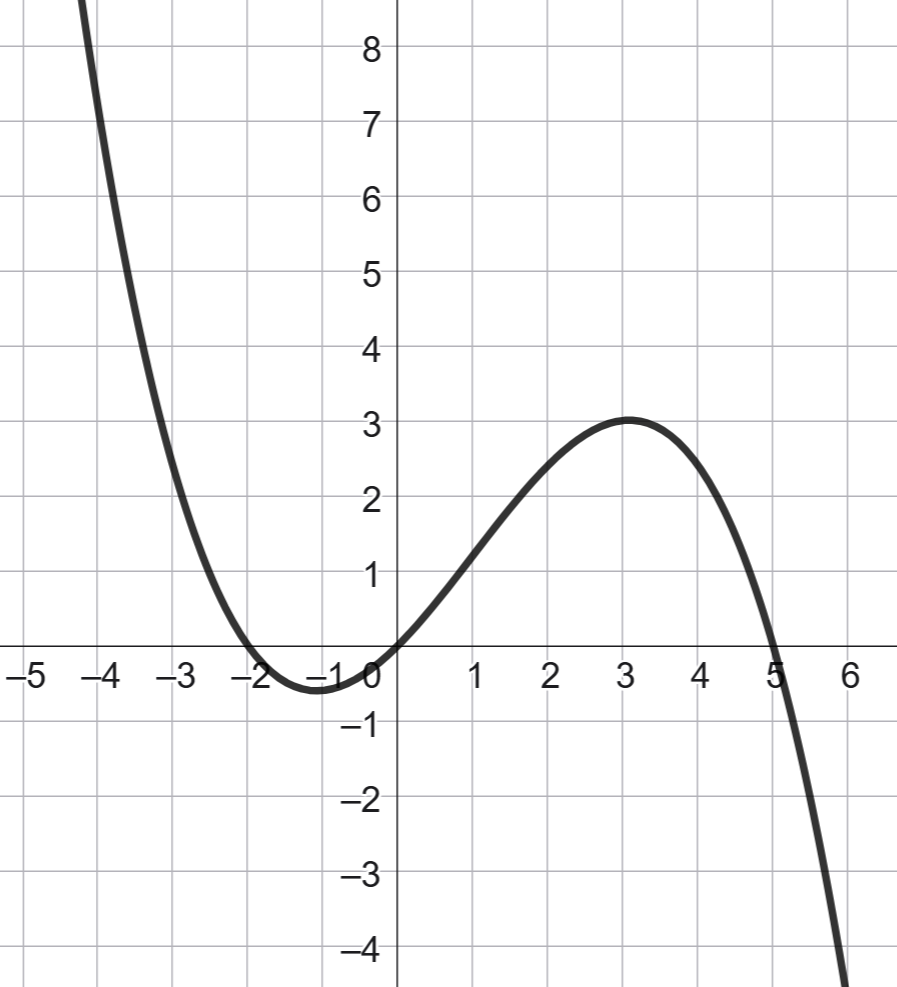
\includegraphics[scale=0.4]{KC3A1}
\end{center}

Answer the following questions. No work required. 

\begin{enumerate}
    \item On what interval(s) is $f(x)$ increasing? On what interval(s) is $f(x)$ decreasing?

    {\large
        \[\text{Increasing: } {\color{blue} (-\infty, -2), (0, 5)}\]
    }

    {\large
        \[\text{Decreasing: } {\color{blue} (-2, 0), (5, \infty)}\]
    }

    \item On what interval(s) is $f(x)$ concave up? On what interval(s) is $f(x)$ concave down?

    {\large
        \[\text{Concave up: } {\color{blue} (-1, 3)}\]
    }

    {\large
        \[\text{Concave down: } {\color{blue} (-\infty, -1), (3, \infty)}\]
    }

    \item At what $x$-values does $f(x)$ have its critical numbers?

    {\large
        \[\text{Critical numbers: } {\color{blue} x=-2, 0, 5}\]
    }

    \item At what $x$-values does $f(x)$ have its inflection points?

    {\large
        \[\text{Inflection points ($x$-value(s) only): } {\color{blue} x=-1, 3}\]
    }
\end{enumerate}

%%%%%%%%%%%%%%%%%%%%%%%%%%%%%%%%%%%%%%%%%%%%%%%%%%%%%
%%%%%%%%%%% END PROBLEM A1 %%%%%%%%%%%%%%%%%%%%%%%%%%
%%%%%%%%%%%%%%%%%%%%%%%%%%%%%%%%%%%%%%%%%%%%%%%%%%%%%

\newpage

%%%%%%%%%%%%%%%%%%%%%%%%%%%%%%%%%%%%%%%%%%%%%%%%%%%%%
%%%%%%%%%%% BEGIN PROBLEM A2 %%%%%%%%%%%%%%%%%%%%%%%%
%%%%%%%%%%%%%%%%%%%%%%%%%%%%%%%%%%%%%%%%%%%%%%%%%%%%%

\item Find the $x$-value(s) of all absolute extrema of  \[f(x)=\dfrac{1}{2}x^4-9x^2+3\] on the interval $[-2, 1]$.

To receive full credit, please provide full justification of why there's an absolute max/min occurring at the $x$-value(s) you've found, and classify each of them as where an absolute maximum or absolute minimum occurs.

You are required to use a method we've learned in our course, such as the first derivative test, the second derivative test, the close interval method, or the first derivative test for absolute extrema, as a part of your justification. In addition, you need to make sure the method you use is suitable for the question.

 {\color{blue}\textbf{Solution:} 
    $f'(x)=2x^3-18x$

    If $f'(x)=0$, we get $2x^3-18x=2x(x^2-9)=2x(x+3)(x-3)=0$, so $x=-3, 0, 3$.

    There's no $x$-value that makes $f'$ DNE, since $f'$ is a polynomial and is defined for all real numbers.

    So the only critical number of $f$ in the interval $[-2, 1]$ is $x=0$.

    We look for values of $f(x)$ at this critical number, as well as the endpoints of the interval of interest.
    
    
    \begin{table}[h!]
        \centering
        \color{blue}
        \begin{tabular}{c|c}
           $x$  & $f(x)$ \\\hline
            $-2$ & $\dfrac{1}{2}\cdot 16-9\cdot 4+3=-25$\\
            $0$ & $3$\\
            $1$ & $\dfrac{1}{2}-9+3=-\dfrac{11}{2}$\\
        \end{tabular}\
    \end{table}
    By comparing these $f(x)$ values, we conclude that on the interval $[-2, 1]$, the function $f(x)$ has its absolute maximum value at $x=0$ and has its absolute minimum value at $x=-2$.

}

{\color{orange} Please note that, the first derivative test and the second derivative test are not suitable for this problem, since they are tests for local extrema, while this problem is asking for absolute extrema.

The first derivative test for absolute extrema does test for absolute extrema, but it would only give one of absolute maximum and absolute minimum, not both. Since this problem is asking for all absolute extrema, using the first derivative test for absolute extrema only would not be sufficient. 

The close interval method is the only method that is sufficient for this problem, which is why we use it here.}

%%%%%%%%%%%%%%%%%%%%%%%%%%%%%%%%%%%%%%%%%%%%%%%%%%%%%
%%%%%%%%%%% END PROBLEM A2 %%%%%%%%%%%%%%%%%%%%%%%%%%
%%%%%%%%%%%%%%%%%%%%%%%%%%%%%%%%%%%%%%%%%%%%%%%%%%%%%

\newpage

%%%%%%%%%%%%%%%%%%%%%%%%%%%%%%%%%%%%%%%%%%%%%%%%%%%%%
%%%%%%%%%%% BEGIN PROBLEM A3 %%%%%%%%%%%%%%%%%%%%%%%%
%%%%%%%%%%%%%%%%%%%%%%%%%%%%%%%%%%%%%%%%%%%%%%%%%%%%%

\item You have 800 ft of fencing to make a four-sided rectangular pen for cattle. The dimensions of the pen are $x$ ft by $y$ ft, as demonstrated in the figure below.

One side of the pen is along a river. To reinforce the pen and avoid cattle falling into the river, this side of the pen requires \textbf{twice as much} of the material as the other three sides. 

What are the dimensions of the rectangular pen that maximizes the area?

\begin{center}
    
\includegraphics[scale=0.5]{Fall 2025/KCs/KC3/KC3A3.png}
\end{center}

To receive full credit, make sure to fully justify why the dimensions you've found maximizes the area. 

You are required to use a method we've learned in our course, such as the first derivative test, the second derivative test, the closed interval method, or the first derivative test for absolute extrema, as a part of your justification. In addition, you need to make sure the method you use is suitable for the question.

\vspace{.2in}

{\color{blue}
\textbf{SOLUTION:} We want to maximize the area, which is $xy$ $\text{ft}^2$.  This is a function of two variables, so we need to rewrite it in terms of one variable.

Since the side along the river requires double fencing, the total fencing for the rectangle is $x + y + 2x + y = 3x + 2y$ ft.  This must equal 800 ft, so we have $$ 3x+2y = 800 \quad \Rightarrow \quad 2y = 800 - 3x \quad  \Rightarrow \quad y = \frac{800 - 3x}{2} = 400 - \frac32 x.$$  We can substitute this expression for $y$ in the area to get that the area is $x (400 - \frac32 x) = 400x - \frac32 x^2$ $\text{ft}^2$.  This now depends on $x$ only, so we can call it $A(x)$.

We need to specify the domain for $A(x)$.  What is the feasible range of possibilities for $x$?  If we allow the pen to have zero length or width, we get the boundary cases $x=0$ and $y=0$.  Note that $y=0$ implies that $x = \frac{800}{3}$ from our equation $3x+2y = 800$.  Thus it's reasonable to say that the domain is $[0, \frac{800}{3}]$.  (It would also be reasonable to insist that the pen be an actual rectangle, not a line segment, making the domain $(0, \frac{800}{3})$.  For the moment let's take $[0, \frac{800}{3}]$.)

We want to find the absolute maximum of the continuous function $A(x) = 400x - \frac32 x^2$ on its domain, which is a closed bounded interval.  We may use the closed interval method.

To find critical values, see where $A'(x) = 0$ or $A'(x)$ DNE.  We have $A'(x) = 400 - 3x$, which exists everywhere.  Setting $A'(x) = 0$ gives $x = \frac{400}{3}$, a critical value which lies in the domain.  We text the endpoints and the critical value:
$$ A(0) = 0, \qquad A\left(\frac{400}{3}\right) =\left(\frac{400}{3}\right)\left(400 - \frac32 \left(\frac{400}{3}\right)\right) = \frac{80000}{3}, \qquad A\left(\frac{800}{3}\right) = 0.$$
The absolute maximum is the largest of these values, occurring when $\boxed{x = \frac{400}{3} \text{ ft}}$ and, using $y= 400 - \frac32 x$, $\boxed{y = 200 \text{ ft}}$.  (We are not asked for the area itself, which is   $\frac{80000}{3} \text{ ft}^2$.)

\textbf{Alternative.} It is also possible to do the last part of this problem via the first derivative test for absolute extrema, since there is one critical value $\frac{400}{3}$ in the domain interval $[0, \frac{800}{3}]$.

We make a sign chart for $A'(x) = 400-3x$ by plugging in numbers from the two subintervals $(0,\frac{400}{3})$ and $(\frac{400}{3}, \frac{800}{3})$. $A'(1) = 397 > 0$; $A'(200) = -200 < 0$.  This means $A$ is increasing on $(0,\frac{400}{3})$ and decreasing on $(\frac{400}{3}, \frac{800}{3})$.  By the first derivative test for absolute extrema, $A$ has its absolute maximum when $\boxed{x = \frac{400}{3} \text{ ft}}$ and, using $y= 400 - \frac32 x$, $\boxed{y = 200 \text{ ft}}$.

This approach also works (and is the only valid option) if the domain is taken to be $(0, \frac{800}{3})$, as mentioned above.



}

%%%%%%%%%%%%%%%%%%%%%%%%%%%%%%%%%%%%%%%%%%%%%%%%%%%%%
%%%%%%%%%%% END PROBLEM A3 %%%%%%%%%%%%%%%%%%%%%%%%%%
%%%%%%%%%%%%%%%%%%%%%%%%%%%%%%%%%%%%%%%%%%%%%%%%%%%%%

\newpage

%%%%%%%%%%%%%%%%%%%%%%%%%%%%%%%%%%%%%%%%%%%%%%%%%%%%%
%%%%%%%%%%% BEGIN PROBLEM I1 %%%%%%%%%%%%%%%%%%%%%%%%
%%%%%%%%%%%%%%%%%%%%%%%%%%%%%%%%%%%%%%%%%%%%%%%%%%%%%

\item 

\begin{enumerate}
    \item The amount of waste a company produces (in tons per week) $t$ weeks since the beginning of 2024 is represented by $W(t)$.
    
    Explain the meaning of the following expression in this context. Make sure to include units.

    \[\int_5^{12}W(t)\,dt=97\]

    {\color{blue}Solution: The net change in the amount of waste a company produced between 5 weeks and 12 weeks since the beginning of 2024 is 97 tons.
    
    OR The total amount of waste a company produced between 5 weeks and 12 weeks since the beginning of 2024 is 97 tons.}

    \vfill

    \item The total number of COVID-19 cases in California is increasing at a rate of $r(t)$ cases per day on day $t$, where $t=1$ represents the end of the day of April 1, 2020.
    
    Suppose there are $7436$ cases at the end of the day on April 1, 2020. Write down an expression involving a definite integral that represents the total number of COVID 19 cases in California at the end of the day on April 20, 2020.

    {\color{blue}Solution: $$7436 + \int_1^{20} r(t) dt$$}

    \vfill
\end{enumerate}

%%%%%%%%%%%%%%%%%%%%%%%%%%%%%%%%%%%%%%%%%%%%%%%%%%%%%
%%%%%%%%%%% END PROBLEM I1 %%%%%%%%%%%%%%%%%%%%%%%%%%
%%%%%%%%%%%%%%%%%%%%%%%%%%%%%%%%%%%%%%%%%%%%%%%%%%%%%

\newpage

%%%%%%%%%%%%%%%%%%%%%%%%%%%%%%%%%%%%%%%%%%%%%%%%%%%%%
%%%%%%%%%%% BEGIN PROBLEM I2 %%%%%%%%%%%%%%%%%%%%%%%%
%%%%%%%%%%%%%%%%%%%%%%%%%%%%%%%%%%%%%%%%%%%%%%%%%%%%%

\item The graph of $f(x)$ is given below.

\begin{center}
    \begin{tikzpicture}[scale=1.25]
          \begin{axis}[
            xlabel={$x$},
            %grid = major,
            xtick       = {1,2,3,4,5,6,7,8,9},
            xticklabels = {$1$,$2$,$3$,$4$,$5$,$6$,$7$,$8$,$9$},
            ytick       = {-3, -2, -1, 0,1,2,3,4},
            yticklabels = {$-3$, $-2$, $-1$, $0$,$1$,$2$,$3$,$4$},
            samples     = 320,
            domain      = -1:9.5,
            restrict y to domain=-3.5:2.5,
            xmin = -0.5, xmax = 9.5,
            ymin = -3.5, ymax = 4.5,
            height=2.1in, width=2.7in,
            grid=both, grid style=dashed
          ]
          \draw[ultra thick, red,--] (-2/3,1/3) -- (2,3) -- (3,3) -- (7, -3) -- (9.5, -0.5);
          \node at (4,3) {$f(x)$};
          \end{axis}
    \end{tikzpicture}
    \end{center}

For any area calculation for this question, please use the respective formula provided on the following page, instead of counting squares. Please show all work.

\begin{enumerate}
    \item Find $\displaystyle\int_0^3 f(x)\,dx$.\\
    {\color{blue}%
    Solution: The integral from $0$ to $3$ corresponds to the area under $f(x)$ from $x=0$ to $x=3$. 

    Break the interval into segments according to the graph using the ``break apart" property:
\[\int_0^3 f(x)\,dx = \int_0^2 f(x)\,dx + \int_2^3 f(x)\,dx\]
    \[
    \int_0^2 f(x)\,dx = \text{area of triangle with base 2, height 2} = \frac{1}{2}\cdot 2 \cdot 2 = 2\] \text{ $+$ two squares with base = height = 1. So we add an area of 2 (one for each square). Hence,}
\[\int_0^2 f(x)\,dx = 2 + 2 = 4\]
    \[
    \int_2^3 f(x)\,dx = \text{area of rectangle with width 1 and height 3} = 1\cdot 3 = 3.
    \]
Hence, 
  \[\int_0^3 f(x)\,dx = \int_0^2 f(x)\,dx + \int_2^3 f(x)\,dx = 4 + 3 = 7\]  
    }
    \item Find $\displaystyle\int_2^7 f(x)\,dx$.\\
 {\color{blue}%
    Solution: The integral from $2$ to $7$ corresponds to the area under $f(x)$ from $x=2$ to $x=7$. 

    Break the interval into segments according to the graph using the ``Break Apart Property":
\[\int_2^7 f(x)\,dx = \int_2^3 f(x)\,dx + \int_3^5 f(x)\,dx + \int_5^7 f(x)\,dx\]
We already calculated $\int_2^3 f(x)\,dx = 3$ in part a). Now, $\int_3^5 f(x)\,dx$ is another triangle with base = 2 and height = 3. So, $\int_3^5 f(x)\,dx  = \dfrac{1}{2} \cdot 2 \cdot 3 = 3$. As for, $\int_5^7 f(x)\,dx$, that is again a triangle with base = 2 and height = 3. However, since the y-values are below the x-axis, this area will be negated. So, $\int_5^7 f(x)\,dx =  -\dfrac{1}{2} \cdot 2 \cdot 3 = -3$. Hence, 
\[\int_2^7 f(x)\,dx = \int_2^3 f(x)\,dx + \int_3^5 f(x)\,dx + \int_5^7 f(x)\,dx = 3 + 3 - 3 = 3.\]
Note the $\int_3^7 f(x)\,dx$ contributed nothing to the net area since the area between the graph and the x-axis between 3 and 5 was cancelled out by the area between the graph and the x-axis between 5 and 7.
    }
    \item Suppose $\displaystyle\int_{3}^{-5} f(x)\,dx=7$. 
    
    Find the value of $\displaystyle\int_{-5}^{0} f(x)\,dx$.\\
{\color{blue}%
Solution: Using the ``reverse limits" property, we see that
$\displaystyle\int_{-5}^{3} f(x)\,dx=-7$. We already calculates $\displaystyle\int_{0}^{3} f(x)\,dx=7$ in a). Now, use the ``break apart property" to observe:

\[
    \displaystyle\int_{-5}^{3} f(x)\,dx = \displaystyle\int_{-5}^{0} f(x)\,dx + \displaystyle\int_{0}^{3} f(x)\,dx \]
    or
    \[-7 = \displaystyle\int_{-5}^{0} f(x)\,dx + 7.\] Solving for $\displaystyle\int_{-5}^{0} f(x)\,dx$, we get 
    \[\displaystyle\int_{-5}^{0} f(x)\,dx = -7 -7 = -14.\]
}
    \vfill
\end{enumerate}

%%%%%%%%%%%%%%%%%%%%%%%%%%%%%%%%%%%%%%%%%%%%%%%%%%%%%
%%%%%%%%%%% END PROBLEM I2 %%%%%%%%%%%%%%%%%%%%%%%%%%
%%%%%%%%%%%%%%%%%%%%%%%%%%%%%%%%%%%%%%%%%%%%%%%%%%%%%

\newpage

\begin{center}
{\bf DO NOT REMOVE THIS SHEET FROM YOUR EXAM PACKET}
\end{center}

\begin{center}
    \begin{tabular}{ r | c | l }
    {\bf Description} & {\bf Formula} & {\bf Variables}\\
    \hline
    area of a square & $A=s^2$ & $s=$ side length\\
    \hline
    area of a rectangle & $A=lw$ & $l=$ length, $w=$ width\\
    \hline
    area of a triangle & $A=\frac12bh$ & $b=$ base, $h=$ height\\
    \hline
    area of a circle & $A=\pi r^2$ & $r=$ radius\\
    \hline
    volume of a rectangular box & $V=lwh$ & $l=$ length, $w=$ width, $h=$ height\\
    \hline
    %volume of a circular cylinder & $V=\pi r^2 h$ & $r=$ radius, $h=$ height\\
    %\hline
    %volume of a sphere & $V=\frac43\pi r^3$ & $r=$ radius\\
    %\hline
    revenue & $R(x) = p\cdot x = p\cdot Q$ & $p=$ unit price, $x=Q=$ quantity sold\\
    \hline
    profit & $P(x) = R(x) - C(x)$ & $R(x)=$ revenue, $C(x)=$ cost\\
    \hline
    average cost & $\overline C(x) = \frac{C(x)}{x}$ & $C(x)=$ cost\\
    \end{tabular}
\end{center}

\begin{center}
{\bf DO NOT REMOVE THIS SHEET FROM YOUR EXAM PACKET}
\end{center}

\newpage

This page is left blank intentionally.\\

Use this page if you need additional space to write your solutions to any problem. \\

If you wish this page graded, you must refer to this page on \textbf{the original page} of the problem. Otherwise, your grader will NOT consider your work on this page.

\end{enumerate}

\end{document}